\documentclass[]{report}
\usepackage{lmodern}
\usepackage{amssymb,amsmath}
\usepackage{ifxetex,ifluatex}
\usepackage{fixltx2e} % provides \textsubscript
\ifnum 0\ifxetex 1\fi\ifluatex 1\fi=0 % if pdftex
  \usepackage[T1]{fontenc}
  \usepackage[utf8]{inputenc}
\else % if luatex or xelatex
  \ifxetex
    \usepackage{mathspec}
  \else
    \usepackage{fontspec}
  \fi
  \defaultfontfeatures{Ligatures=TeX,Scale=MatchLowercase}
\fi
% use upquote if available, for straight quotes in verbatim environments
\IfFileExists{upquote.sty}{\usepackage{upquote}}{}
% use microtype if available
\IfFileExists{microtype.sty}{%
\usepackage{microtype}
\UseMicrotypeSet[protrusion]{basicmath} % disable protrusion for tt fonts
}{}
\usepackage{hyperref}
\hypersetup{unicode=true,
            pdftitle={Data 624: Homework II},
            pdfauthor={Vinicio Haro; Sang Yoon (Andy) Hwang; Julian McEachern; Jeremy O'Brien; Bethany Poulin},
            pdfborder={0 0 0},
            breaklinks=true}
\urlstyle{same}  % don't use monospace font for urls
\usepackage{color}
\usepackage{fancyvrb}
\newcommand{\VerbBar}{|}
\newcommand{\VERB}{\Verb[commandchars=\\\{\}]}
\DefineVerbatimEnvironment{Highlighting}{Verbatim}{commandchars=\\\{\}}
% Add ',fontsize=\small' for more characters per line
\usepackage{framed}
\definecolor{shadecolor}{RGB}{248,248,248}
\newenvironment{Shaded}{\begin{snugshade}}{\end{snugshade}}
\newcommand{\AlertTok}[1]{\textcolor[rgb]{0.94,0.16,0.16}{#1}}
\newcommand{\AnnotationTok}[1]{\textcolor[rgb]{0.56,0.35,0.01}{\textbf{\textit{#1}}}}
\newcommand{\AttributeTok}[1]{\textcolor[rgb]{0.77,0.63,0.00}{#1}}
\newcommand{\BaseNTok}[1]{\textcolor[rgb]{0.00,0.00,0.81}{#1}}
\newcommand{\BuiltInTok}[1]{#1}
\newcommand{\CharTok}[1]{\textcolor[rgb]{0.31,0.60,0.02}{#1}}
\newcommand{\CommentTok}[1]{\textcolor[rgb]{0.56,0.35,0.01}{\textit{#1}}}
\newcommand{\CommentVarTok}[1]{\textcolor[rgb]{0.56,0.35,0.01}{\textbf{\textit{#1}}}}
\newcommand{\ConstantTok}[1]{\textcolor[rgb]{0.00,0.00,0.00}{#1}}
\newcommand{\ControlFlowTok}[1]{\textcolor[rgb]{0.13,0.29,0.53}{\textbf{#1}}}
\newcommand{\DataTypeTok}[1]{\textcolor[rgb]{0.13,0.29,0.53}{#1}}
\newcommand{\DecValTok}[1]{\textcolor[rgb]{0.00,0.00,0.81}{#1}}
\newcommand{\DocumentationTok}[1]{\textcolor[rgb]{0.56,0.35,0.01}{\textbf{\textit{#1}}}}
\newcommand{\ErrorTok}[1]{\textcolor[rgb]{0.64,0.00,0.00}{\textbf{#1}}}
\newcommand{\ExtensionTok}[1]{#1}
\newcommand{\FloatTok}[1]{\textcolor[rgb]{0.00,0.00,0.81}{#1}}
\newcommand{\FunctionTok}[1]{\textcolor[rgb]{0.00,0.00,0.00}{#1}}
\newcommand{\ImportTok}[1]{#1}
\newcommand{\InformationTok}[1]{\textcolor[rgb]{0.56,0.35,0.01}{\textbf{\textit{#1}}}}
\newcommand{\KeywordTok}[1]{\textcolor[rgb]{0.13,0.29,0.53}{\textbf{#1}}}
\newcommand{\NormalTok}[1]{#1}
\newcommand{\OperatorTok}[1]{\textcolor[rgb]{0.81,0.36,0.00}{\textbf{#1}}}
\newcommand{\OtherTok}[1]{\textcolor[rgb]{0.56,0.35,0.01}{#1}}
\newcommand{\PreprocessorTok}[1]{\textcolor[rgb]{0.56,0.35,0.01}{\textit{#1}}}
\newcommand{\RegionMarkerTok}[1]{#1}
\newcommand{\SpecialCharTok}[1]{\textcolor[rgb]{0.00,0.00,0.00}{#1}}
\newcommand{\SpecialStringTok}[1]{\textcolor[rgb]{0.31,0.60,0.02}{#1}}
\newcommand{\StringTok}[1]{\textcolor[rgb]{0.31,0.60,0.02}{#1}}
\newcommand{\VariableTok}[1]{\textcolor[rgb]{0.00,0.00,0.00}{#1}}
\newcommand{\VerbatimStringTok}[1]{\textcolor[rgb]{0.31,0.60,0.02}{#1}}
\newcommand{\WarningTok}[1]{\textcolor[rgb]{0.56,0.35,0.01}{\textbf{\textit{#1}}}}
\usepackage{graphicx,grffile}
\makeatletter
\def\maxwidth{\ifdim\Gin@nat@width>\linewidth\linewidth\else\Gin@nat@width\fi}
\def\maxheight{\ifdim\Gin@nat@height>\textheight\textheight\else\Gin@nat@height\fi}
\makeatother
% Scale images if necessary, so that they will not overflow the page
% margins by default, and it is still possible to overwrite the defaults
% using explicit options in \includegraphics[width, height, ...]{}
\setkeys{Gin}{width=\maxwidth,height=\maxheight,keepaspectratio}
\IfFileExists{parskip.sty}{%
\usepackage{parskip}
}{% else
\setlength{\parindent}{0pt}
\setlength{\parskip}{6pt plus 2pt minus 1pt}
}
\setlength{\emergencystretch}{3em}  % prevent overfull lines
\providecommand{\tightlist}{%
  \setlength{\itemsep}{0pt}\setlength{\parskip}{0pt}}
\setcounter{secnumdepth}{0}

%%% Use protect on footnotes to avoid problems with footnotes in titles
\let\rmarkdownfootnote\footnote%
\def\footnote{\protect\rmarkdownfootnote}

%%% Change title format to be more compact
\usepackage{titling}

% Create subtitle command for use in maketitle
\providecommand{\subtitle}[1]{
  \posttitle{
    \begin{center}\large#1\end{center}
    }
}

\setlength{\droptitle}{-2em}

  \title{Data 624: Homework II}
    \pretitle{\vspace{\droptitle}\centering\huge}
  \posttitle{\par}
  \subtitle{Group Two}
  \author{Vinicio Haro \\ Sang Yoon (Andy) Hwang \\ Julian McEachern \\ Jeremy O'Brien \\ Bethany Poulin}
    \preauthor{\centering\large\emph}
  \postauthor{\par}
      \predate{\centering\large\emph}
  \postdate{\par}
    \date{16 December 2019}

% set plain style for page numbers
\pagestyle{plain}
\raggedbottom

% change font
\usepackage{fontspec}
\setmainfont{Arial}

% create color block quotes
\usepackage[dvipsnames]{xcolor}
\usepackage{tcolorbox}     
\newtcolorbox{question}[1]{colback=white, colframe=Emerald ,fonttitle=\bfseries, title=#1}

\newtcolorbox{subquestion}[1]{colback=white,colframe=white, coltitle=Emerald!75!black, detach title, before upper={\tcbtitle\quad\hangindent7mm}, title={#1},fonttitle=\bfseries, fontupper=\bfseries}

% remove "chapter" from chapter title
\usepackage{titlesec}
\titleformat{\chapter}
  {\normalfont\LARGE\bfseries}{\thechapter}{1em}{}
\titlespacing*{\chapter}{0pt}{3.5ex plus 1ex minus .2ex}{2.3ex plus .2ex}

% wrap text
\usepackage{geometry}[textwidth=6in]

% kable 
\usepackage{tabu}
\usepackage{float} 

% multicolumn
\usepackage{multicol}
\usepackage{booktabs}
\usepackage{longtable}
\usepackage{array}
\usepackage{multirow}
\usepackage{wrapfig}
\usepackage{float}
\usepackage{colortbl}
\usepackage{pdflscape}
\usepackage{tabu}
\usepackage{threeparttable}
\usepackage{threeparttablex}
\usepackage[normalem]{ulem}
\usepackage{makecell}
\usepackage{xcolor}

\begin{document}
\maketitle

{
\setcounter{tocdepth}{2}
\tableofcontents
}
\hypertarget{dependencies}{%
\section{Dependencies}\label{dependencies}}

\begin{Shaded}
\begin{Highlighting}[]
\CommentTok{# Processing}
\KeywordTok{libraries}\NormalTok{(}\StringTok{"mice"}\NormalTok{, }\StringTok{"AppliedPredictiveModeling"}\NormalTok{, }\StringTok{"tidyverse"}\NormalTok{, }
    \StringTok{"caret"}\NormalTok{, }\StringTok{"pls"}\NormalTok{, }\StringTok{"recipes"}\NormalTok{, }\StringTok{"corrplot"}\NormalTok{)}

\CommentTok{# Formatting Libraries}

\KeywordTok{libraries}\NormalTok{(}\StringTok{"default"}\NormalTok{, }\StringTok{"knitr"}\NormalTok{, }\StringTok{"kableExtra"}\NormalTok{)}

\CommentTok{# Plotting Libraries}
\KeywordTok{libraries}\NormalTok{(}\StringTok{"ggplot2"}\NormalTok{, }\StringTok{"grid"}\NormalTok{, }\StringTok{"ggfortify"}\NormalTok{)}
\end{Highlighting}
\end{Shaded}

\hypertarget{AS-1}{%
\chapter*{Assignment 1}\label{AS-1}}
\addcontentsline{toc}{chapter}{Assignment 1}

\addcontentsline{toc}{section}{Kuhn and Johnson 6.3}

\begin{question}{Kuhn and Johnson 6.3}A chemical manufacturing process for a pharmaceutical product was discussed in Sect.1.4. In this problem, the objective is to understand the relationship between biological measurements of the raw materials (predictors), measurements of the manufacturing process (predictors), and the response of product yield. Biological predictors cannot be changed but can be used to assess the quality of the raw material before processing. On the other hand, manufacturing process predictors can be changed in the manufacturing process. Improving product yield by 1\% will boost revenue by approximately one hundred thousand dollars per batch:\end{question}

\begin{subquestion}{(a).}Start R and use these commands to load the data:
\end{subquestion}

\begin{Shaded}
\begin{Highlighting}[]
\KeywordTok{data}\NormalTok{(}\StringTok{"ChemicalManufacturingProcess"}\NormalTok{)}
\end{Highlighting}
\end{Shaded}

The matrix processPredictors contains the 57 predictors (12 describing
the input biological material and 45 describing the process predictors)
for the 176 manufacturing runs. yield contains the percent yield for
each run.

\begin{subquestion}{(b).} A small percentage of cells in the predictor set contain missing values. Use an imputation function to fill in these missing values (e.g., see Sect. 3.8). 
\end{subquestion}

There are 28 predictor variables with 106 missing values within the
\texttt{ChemicalManufacturingProcess} (CMP) dataset. The \texttt{mice}
function from the \texttt{mice} package can be used to impute
multivariate missing data. The method applies a unique model to each
variable to conduct multiple imputations. After running the function, we
apply the \texttt{complete} function to fill in the missing data. There
are now 0 missing values within the dataset.

\begin{subquestion}{(c).} Split the data into a training and a test set, pre-process the data, and tune a model of your choice from this chapter. What is the optimal value of the performance metric? 
\end{subquestion}

For this question, we decided to use a partial least squares (pls)
method to model the data. We created evaluation method using the
\texttt{createDataPartition} from the \texttt{caret} package, where 80\%
of the CMP data was randomly selected for training and 20\% for testing
purposes. We built two models to compare the effect pre-processing and
tuning had on the fitting the data. Our pre-processing methods involved
applying a principal component analysis (pca). In doing so, we
recognized one of our variables, \texttt{BiologicalMaterial08}, had
near-zero variance so we applied a recipe to filter that variable. We
also applied training controls to resample the data over 5 folds.

The pre-processing components included the following:

\begin{verbatim}
Created from 144 samples and 56 variables

Pre-processing:
  - centered (56)
  - ignored (0)
  - principal component signal extraction (56)
  - scaled (56)

PCA needed 25 components to capture 95 percent of the variance
\end{verbatim}

We found that this approach helped improve model accuracy metrics. The
optimal value of the performance metric for our model with
transformations was 1.53, whereas the optimal value for the model
without pre-processing was 1.77.

\textbf{PLS Model - No Pre-Processing}

\begin{verbatim}
Partial Least Squares 

144 samples
 57 predictor

No pre-processing
Resampling: Bootstrapped (25 reps) 
Summary of sample sizes: 144, 144, 144, 144, 144, 144, ... 
Resampling results across tuning parameters:

  ncomp  RMSE      Rsquared    MAE     
  1      1.771420  0.12809343  1.417675
  2      2.158868  0.11869755  1.496848
  3      3.581090  0.09634691  1.752045
  4      6.930771  0.08060499  2.207104
  5      5.680859  0.15421739  1.915612

RMSE was used to select the optimal model using the smallest value.
The final value used for the model was ncomp = 1.
\end{verbatim}

\textbf{PLS Model - With Pre-Processing}

\begin{verbatim}
Partial Least Squares 

144 samples
 56 predictor

Pre-processing: principal component signal extraction (56), centered
 (56), scaled (56) 
Resampling: Cross-Validated (5 fold) 
Summary of sample sizes: 114, 116, 116, 115, 115 
Resampling results across tuning parameters:

  ncomp  RMSE      Rsquared   MAE     
  1      1.519177  0.4249250  1.160602
  2      1.793880  0.4441069  1.153173
  3      1.525966  0.5180790  1.083496
  4      1.475197  0.5362954  1.062071
  5      1.511131  0.5224443  1.068680

RMSE was used to select the optimal model using the smallest value.
The final value used for the model was ncomp = 4.
\end{verbatim}

\begin{subquestion}{(d).} Predict the response for the test set. What is the value of the performance metric and how does this compare with the resampled performance metric on the training set? 
\end{subquestion}

The RMSE for the test data set was 1.22, which was slightly higher than
when we fitted the model on the train data (RMSE: 1.53). We compared the
test predictions with the observed data below:

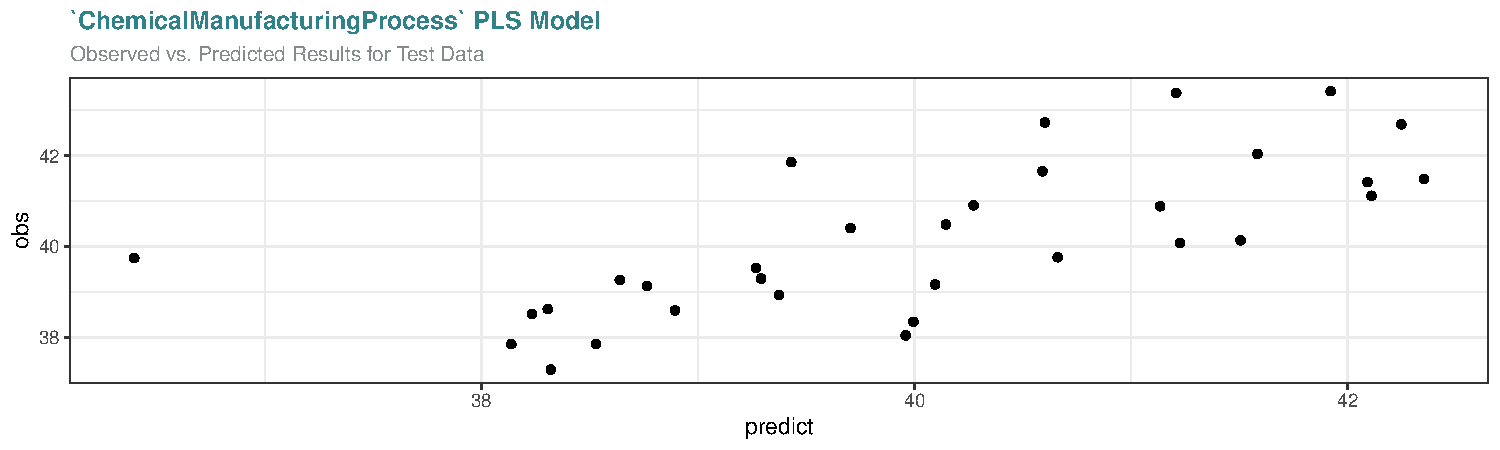
\includegraphics{Format_Test_files/figure-latex/kj-6.3d-1-1.pdf}

\begin{subquestion}{(e).} Which predictors are most important in the model you have trained? Do either the biological or process predictors dominate the list? 
\end{subquestion}

The \texttt{varImp} function allows us to see the importance of our
model's principal components. Biological predictors make up 8, or 80\%,
of our top 10 variables. The following plot shows the ranks of
importance of our model's principal components:

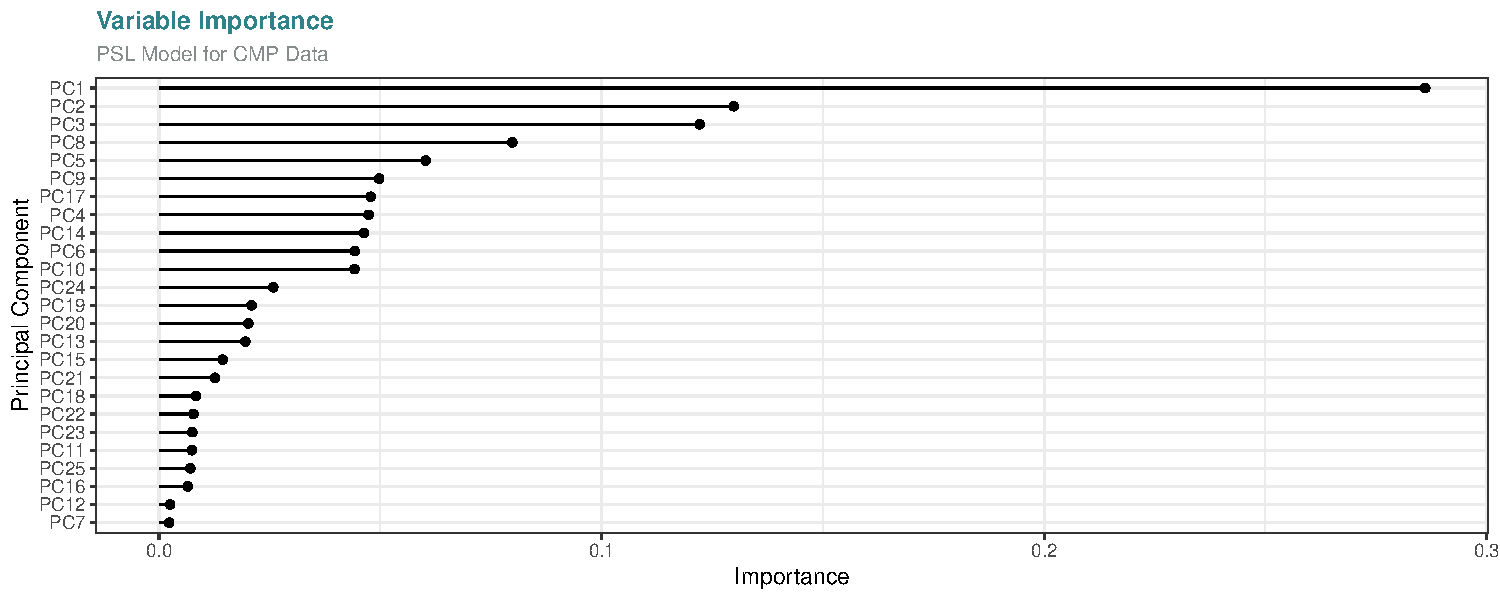
\includegraphics{Format_Test_files/figure-latex/kj-6.3e-1-1.pdf}

\begin{subquestion}{(f).} Explore the relationships between each of the top predictors and the response. How could this information be helpful in improving yield in future runs of the manufacturing process?
\end{subquestion}

Below, we looked at the correlation between our top predictor variables
with our response variable:

\begin{table}[H]
\centering
\begin{tabular}{l|r}
\hline
BiologicalMaterial01 & 0.3427280\\
\hline
\rowcolor{gray!6}  BiologicalMaterial03 & 0.4827276\\
\hline
BiologicalMaterial02 & 0.5100752\\
\hline
\rowcolor{gray!6}  BiologicalMaterial09 & 0.1107648\\
\hline
BiologicalMaterial10 & 0.1691056\\
\hline
\rowcolor{gray!6}  BiologicalMaterial12 & 0.4463825\\
\hline
ManufacturingProcess07 & -0.0345109\\
\hline
\rowcolor{gray!6}  BiologicalMaterial05 & 0.1626980\\
\hline
BiologicalMaterial06 & 0.5315807\\
\hline
\rowcolor{gray!6}  ManufacturingProcess03 & -0.1325062\\
\hline
\end{tabular}
\end{table}

Both our top manufacturing predictor variables have a negative
correlation coefficient which would be beneficial to examine to improve
yield predictions in future models.

\hypertarget{r-code}{%
\section{R Code}\label{r-code}}

\begin{Shaded}
\begin{Highlighting}[]
\CommentTok{# (6.3a) Load data}
\KeywordTok{data}\NormalTok{(}\StringTok{"ChemicalManufacturingProcess"}\NormalTok{)}

\CommentTok{# (6.3b) Calculate NA Values}
\NormalTok{CMP_NA <-}\StringTok{ }\NormalTok{ChemicalManufacturingProcess }\OperatorTok\StringTok{ }\KeywordTok{select}\NormalTok{(}\OperatorTok{-}\NormalTok{Yield) }\OperatorTok\StringTok{ }
\StringTok{    }\KeywordTok{summarise_all}\NormalTok{(}\KeywordTok{funs}\NormalTok{(}\KeywordTok{sum}\NormalTok{(}\KeywordTok{is.na}\NormalTok{(.)))) }\OperatorTok\StringTok{ }\KeywordTok{t}\NormalTok{() }\OperatorTok\StringTok{ }
\StringTok{    }\KeywordTok{as.data.frame}\NormalTok{() }\OperatorTok\StringTok{ }\KeywordTok{rownames_to_column}\NormalTok{(}\StringTok{"Predictor"}\NormalTok{) }\OperatorTok\StringTok{ }
\StringTok{    }\KeywordTok{filter}\NormalTok{(V1 }\OperatorTok{>}\StringTok{ }\DecValTok{0}\NormalTok{)}

\CommentTok{# Impute NA Values}
\NormalTok{CMP_Impute <-}\StringTok{ }\KeywordTok{mice}\NormalTok{(ChemicalManufacturingProcess, }\DataTypeTok{m =} \DecValTok{5}\NormalTok{, }
    \DataTypeTok{printFlag =}\NormalTok{ F)}
\NormalTok{CMP_DF <-}\StringTok{ }\NormalTok{mice}\OperatorTok{::}\KeywordTok{complete}\NormalTok{(CMP_Impute, }\DecValTok{2}\NormalTok{)}

\CommentTok{# Verify}
\NormalTok{CMP_Verify <-}\StringTok{ }\KeywordTok{sum}\NormalTok{(}\KeywordTok{is.na}\NormalTok{(CMP_DF))}

\CommentTok{# (6.3c) Set random seed}
\KeywordTok{set.seed}\NormalTok{(}\DecValTok{50}\NormalTok{)}

\CommentTok{# Create Partition for Train/Test Splits}
\NormalTok{trainingRows <-}\StringTok{ }\KeywordTok{createDataPartition}\NormalTok{(CMP_DF}\OperatorTok{$}\NormalTok{Yield, }\DataTypeTok{p =} \FloatTok{0.8}\NormalTok{, }
    \DataTypeTok{list =} \OtherTok{FALSE}\NormalTok{)}

\CommentTok{# Split Train/Test Data}
\NormalTok{train <-}\StringTok{ }\NormalTok{CMP_DF[trainingRows, ]}
\NormalTok{test <-}\StringTok{ }\NormalTok{CMP_DF[}\OperatorTok{-}\NormalTok{trainingRows, ]}

\CommentTok{# Create model function}
\NormalTok{fit_pls_}\DecValTok{1}\NormalTok{ <-}\StringTok{ }\KeywordTok{train}\NormalTok{(Yield }\OperatorTok{~}\StringTok{ }\NormalTok{., }\DataTypeTok{data =}\NormalTok{ train, }\DataTypeTok{method =} \StringTok{"pls"}\NormalTok{, }
    \DataTypeTok{tuneLength =} \DecValTok{5}\NormalTok{)}

\CommentTok{# Pre-Process Recipe}
\NormalTok{rec <-}\StringTok{ }\NormalTok{recipes}\OperatorTok{::}\KeywordTok{recipe}\NormalTok{(CMP_DF, Yield }\OperatorTok{~}\StringTok{ }\NormalTok{.)}
\NormalTok{rec <-}\StringTok{ }\NormalTok{rec }\OperatorTok\StringTok{ }\KeywordTok{step_nzv}\NormalTok{(}\KeywordTok{all_predictors}\NormalTok{(), }\DataTypeTok{options =} \KeywordTok{list}\NormalTok{(}\DataTypeTok{freq_cut =} \DecValTok{95}\OperatorTok{/}\DecValTok{5}\NormalTok{, }
    \DataTypeTok{unique_cut =} \DecValTok{10}\NormalTok{))}
\NormalTok{prep_rec =}\StringTok{ }\KeywordTok{prep}\NormalTok{(rec, }\DataTypeTok{training =}\NormalTok{ CMP_DF)}
\NormalTok{CMP_DF_TF =}\StringTok{ }\KeywordTok{bake}\NormalTok{(prep_rec, CMP_DF)}

\CommentTok{# Create Partition for Train/Test Splits}
\NormalTok{trainingRows <-}\StringTok{ }\KeywordTok{createDataPartition}\NormalTok{(CMP_DF_TF}\OperatorTok{$}\NormalTok{Yield, }
    \DataTypeTok{p =} \FloatTok{0.8}\NormalTok{, }\DataTypeTok{list =} \OtherTok{FALSE}\NormalTok{)}

\CommentTok{# Split Train/Test Data}
\NormalTok{train <-}\StringTok{ }\NormalTok{CMP_DF_TF[trainingRows, ]}
\NormalTok{test <-}\StringTok{ }\NormalTok{CMP_DF_TF[}\OperatorTok{-}\NormalTok{trainingRows, ]}

\CommentTok{# Create model function}
\NormalTok{fit_pls_}\DecValTok{2}\NormalTok{ <-}\StringTok{ }\KeywordTok{train}\NormalTok{(Yield }\OperatorTok{~}\StringTok{ }\NormalTok{., }\DataTypeTok{data =}\NormalTok{ train, }\DataTypeTok{method =} \StringTok{"pls"}\NormalTok{, }
    \DataTypeTok{preProcess =} \StringTok{"pca"}\NormalTok{, }\DataTypeTok{trControl =} \KeywordTok{trainControl}\NormalTok{(}\DataTypeTok{method =} \StringTok{"cv"}\NormalTok{, }
        \DataTypeTok{number =} \DecValTok{5}\NormalTok{), }\DataTypeTok{tuneLength =} \DecValTok{5}\NormalTok{)}

\NormalTok{RMSE_}\DecValTok{1}\NormalTok{ <-}\StringTok{ }\NormalTok{fit_pls_}\DecValTok{1}\OperatorTok{$}\NormalTok{results}\OperatorTok{$}\NormalTok{RMSE[}\DecValTok{1}\NormalTok{]}
\NormalTok{RMSE_}\DecValTok{2}\NormalTok{ <-}\StringTok{ }\NormalTok{fit_pls_}\DecValTok{2}\OperatorTok{$}\NormalTok{results}\OperatorTok{$}\NormalTok{RMSE[}\DecValTok{3}\NormalTok{]}

\CommentTok{# (6.3d) Predict Response}
\NormalTok{predict <-}\StringTok{ }\KeywordTok{predict}\NormalTok{(fit_pls_}\DecValTok{2}\NormalTok{, test)}

\CommentTok{# Performance Metrics}
\NormalTok{test_predict_result <-}\StringTok{ }\KeywordTok{data.frame}\NormalTok{(}\DataTypeTok{obs =}\NormalTok{ test}\OperatorTok{$}\NormalTok{Yield, }
    \DataTypeTok{pred =}\NormalTok{ predict)}

\CommentTok{# summarize results}
\NormalTok{test_predict_accuracy <-}\StringTok{ }\KeywordTok{defaultSummary}\NormalTok{(test_predict_result)}
\NormalTok{RMSE_}\DecValTok{3}\NormalTok{ <-}\StringTok{ }\NormalTok{test_predict_accuracy[[}\DecValTok{1}\NormalTok{]]}

\CommentTok{# plot}
\NormalTok{plot <-}\StringTok{ }\KeywordTok{ggplot}\NormalTok{(test_predict_result, }\KeywordTok{aes}\NormalTok{(obs, predict)) }\OperatorTok{+}\StringTok{ }
\StringTok{    }\KeywordTok{labs}\NormalTok{(}\DataTypeTok{title =} \StringTok{"`ChemicalManufacturingProcess` PLS Model"}\NormalTok{, }
        \DataTypeTok{subtitle =} \StringTok{"Observed vs. Predicted Results for Test Data"}\NormalTok{) }\OperatorTok{+}\StringTok{ }
\StringTok{    }\KeywordTok{geom_point}\NormalTok{() }\OperatorTok{+}\StringTok{ }\KeywordTok{coord_flip}\NormalTok{() }\OperatorTok{+}\StringTok{ }\KeywordTok{theme_bw}\NormalTok{() }\OperatorTok{+}\StringTok{ }\KeywordTok{theme}\NormalTok{()}

\CommentTok{# (6.3e)}
\NormalTok{varimp1 <-}\StringTok{ }\KeywordTok{varImp}\NormalTok{(fit_pls_}\DecValTok{2}\NormalTok{, }\DataTypeTok{scale =}\NormalTok{ F, }\DataTypeTok{useModel =}\NormalTok{ T)}

\NormalTok{varimp2 <-}\StringTok{ }\NormalTok{varimp1}\OperatorTok{$}\NormalTok{importance }\OperatorTok\StringTok{ }\KeywordTok{rownames_to_column}\NormalTok{(}\StringTok{"Principal Component"}\NormalTok{)}

\NormalTok{plot <-}\StringTok{ }\KeywordTok{ggplot}\NormalTok{(varimp2, }\KeywordTok{aes}\NormalTok{(}\DataTypeTok{x =} \KeywordTok{reorder}\NormalTok{(}\StringTok{`}\DataTypeTok{Principal Component}\StringTok{`}\NormalTok{, }
\NormalTok{    Overall), }\DataTypeTok{y =}\NormalTok{ Overall)) }\OperatorTok{+}\StringTok{ }\KeywordTok{geom_point}\NormalTok{() }\OperatorTok{+}\StringTok{ }\KeywordTok{geom_segment}\NormalTok{(}\KeywordTok{aes}\NormalTok{(}\DataTypeTok{x =} \StringTok{`}\DataTypeTok{Principal Component}\StringTok{`}\NormalTok{, }
    \DataTypeTok{xend =} \StringTok{`}\DataTypeTok{Principal Component}\StringTok{`}\NormalTok{, }\DataTypeTok{y =} \DecValTok{0}\NormalTok{, }\DataTypeTok{yend =}\NormalTok{ Overall)) }\OperatorTok{+}\StringTok{ }
\StringTok{    }\KeywordTok{labs}\NormalTok{(}\DataTypeTok{title =} \StringTok{"Variable Importance"}\NormalTok{, }\DataTypeTok{subtitle =} \StringTok{"PSL Model for CMP Data"}\NormalTok{, }
        \DataTypeTok{x =} \StringTok{"Principal Component"}\NormalTok{, }\DataTypeTok{y =} \StringTok{"Importance"}\NormalTok{) }\OperatorTok{+}\StringTok{ }
\StringTok{    }\KeywordTok{coord_flip}\NormalTok{() }\OperatorTok{+}\StringTok{ }\KeywordTok{theme_bw}\NormalTok{() }\OperatorTok{+}\StringTok{ }\KeywordTok{theme}\NormalTok{()}

\NormalTok{varimp_pc <-}\StringTok{ }\NormalTok{train }\OperatorTok\StringTok{ }\KeywordTok{select}\NormalTok{(}\OperatorTok{-}\NormalTok{Yield) }\OperatorTok\StringTok{ }\KeywordTok{select}\NormalTok{(}\DecValTok{1}\NormalTok{, }
    \DecValTok{3}\NormalTok{, }\DecValTok{2}\NormalTok{, }\DecValTok{8}\NormalTok{, }\DecValTok{9}\NormalTok{, }\DecValTok{11}\NormalTok{, }\DecValTok{18}\NormalTok{, }\DecValTok{5}\NormalTok{, }\DecValTok{6}\NormalTok{, }\DecValTok{14}\NormalTok{)}
\NormalTok{bio <-}\StringTok{ }\NormalTok{varimp_pc }\OperatorTok\StringTok{ }\KeywordTok{select}\NormalTok{(}\KeywordTok{starts_with}\NormalTok{(}\StringTok{"Bio"}\NormalTok{)) }\OperatorTok\StringTok{ }
\StringTok{    }\KeywordTok{ncol}\NormalTok{()}

\CommentTok{# (6.3f)}
\NormalTok{top <-}\StringTok{ }\NormalTok{varimp_pc }\OperatorTok\StringTok{ }\KeywordTok{colnames}\NormalTok{()}
\NormalTok{cor <-}\StringTok{ }\KeywordTok{cor}\NormalTok{(train[, top], train}\OperatorTok{$}\NormalTok{Yield, }\DataTypeTok{method =} \StringTok{"pearson"}\NormalTok{)}
\end{Highlighting}
\end{Shaded}


\end{document}
